%====================================================================================================
%----------------------------------------------------------------------------------------------------
% Autor				: Vagner da Silva Bezerra
%----------------------------------------------------------------------------------------------------
% Data de criação	: 10 de Outubro de 2016
%====================================================================================================

\chapter{Fundamentação Teórica}\label{cap:funTeorica}

Neste Capítulo são apresentados os conceitos utilizados neste trabalho de acordo com a literatura estudada. Na seção \ref{sec:falhaErroDefeito} explica-se os conceitos de falha, erro e defeito ou modelo de três universos. Na Seção \ref{sec:radiacao} são descritas as principais fontes de radiação e seus efeitos nos circuitos eletrônicos. Na Seção \ref{sec:denpendabilidade} explica-se o conceito de "dependabilidade". Na Seção \ref{sec:tolerancia} explica-se o conceito de tolerância a falhas e os atributos necessários para que uma falha seja considerada como tal. Na Seção \ref{sec:tecnica} são apresentas as principais técnicas de tolerância a falhas e na Seção \ref{sec:InjecaoDeFalhas} as principais técnicas de injeção de falhas.

\section{Falha, Erro e Defeito} \label{sec:falhaErroDefeito}

Quando aplicado a sistemas digitais os termos falha, erro e defeito possuem significados diferentes. Defeito indica uma incapacidade do sistema executar uma determinada tarefa devido a erros em algum componente do dispositivo ou no ambiente, que por sua vez, são causados por falhas \cite{Nelson:1990}.

Segundo Nelson \cite{Nelson:1990} uma falha é uma condição física anômala. As causas estão associadas a erros de projeto, tais como erros de especificação do sistema: problemas de fabricação; danos causados em algum componente, ferrugem, ou outros tipos de deteriorações; e perturbações externas, como duras condições ambientais, interferência eletromagnética, radiação ionizante, ou má utilização do sistema. Falhas resultantes de erros de projetos e fatores externos são especialmente difíceis de serem protegidos com uma modelagem prévia, porque suas ocorrências e efeitos são difíceis de serem previstos, por exemplo, que o \textit{hardware} utilizado seja exposto a um alto nível de radiação. Já Johnson \cite{Johnson:1984} explica os conceitos de falha, erro e defeito utilizando um modelo de universo, nos quais falhas são associadas ao universo físico, erros ao universo da informação e defeitos ao universo do usuário. 

\begin{figure}[H]
	\centering
	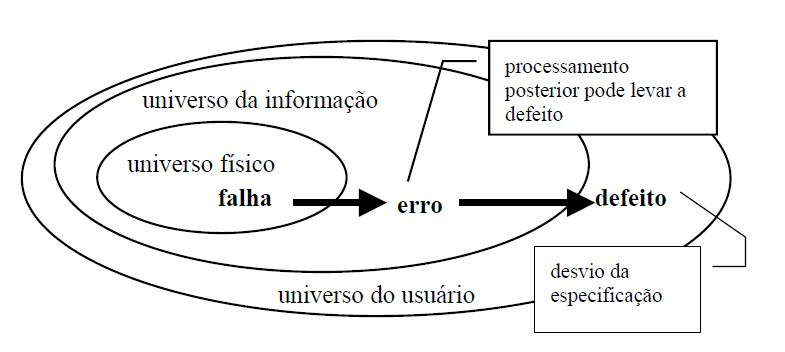
\includegraphics[width=0.7\textwidth]{figuras/modeloUniverso.jpg}
	\caption[Modelo de três universos]{Modelo de 3 universos: falha, erro e defeito. Retirado de Weber \cite{Weber:2002}.}
	\label{Img:modeloUniverso}	
	%width=0.5\textwidth (Tamanho da Imagem)
\end{figure}

Um exemplo de uma falha no universo físico é um chip de memória com uma falha do tipo grudado-em-zero (\textit{stack-at-zero}). Esta falha pode gerar um erro no universo da informação, uma vez que pode-se influenciar uma interpretação equivocada da informação armazenada em um dispositivo eletrônico, alterando o seu valor e como resultado esta alteração se torna um defeito, perceptível ao universo do usuário, no qual o sistema pode negar autorização de embarque para todos os passageiros de um voo \cite{Nelson:1990}. Na Figura \ref{Img:modeloUniverso} é mostrado a simplificação do exemplo anterior.

\section{Principais Fontes de Radiação e seus Efeitos nos Circuitos Eletrônicos} \label{sec:radiacao}

Em 1962 ocorreu uma falha no Satélite de Telecomunicações \textit{Telstar} após um teste nuclear realizado em alta altitude pelos Estados Unidos, surge então a primeira evidência de que a radiação pode perturbar a operação de circuitos eletrônicos \cite{Velazco:2007}. Após este acontecimento, a comunidade científica, agências espaciais e órgãos militares passaram a estudar os efeitos da radiação nos circuitos eletrônicos. Um segundo fato que levou a exploração desse assunto foi a queda de um avião Airbus A320 em fevereiro de 1990 na cidade de Bangalore na Índia, investigações preliminares sugeriram que os computadores de controle poderiam ter realizado algumas especificações segundos antes do início da queda \cite{LaprieAcidente:1990}.

A radiação está presente tanto no espaço quanto na atmosfera, podendo alterar a resposta ou danificar componentes eletrônicos expostos a íons pesados (partículas carregadas), como por exemplo, os transistores. Circuitos eletrônicos podem sofrer efeitos indesejados e as principais partículas responsáveis por isso são prótons, elétrons, nêutrons, íons pesados e partículas alfa, além da radiação eletromagnética (como, por exemplo, raio-x). As principais fontes de radiação de origem espacial são os cinturões de \textit{Van Allen}, os raios cósmicos \cite{Stassinopoulos:1988} e a atividade solar \cite{Boudenot:2007}. Estas partículas podem gerar pulsos transitórios nos transistores que dependendo de sua amplitude em tensão, corrente e duração podem ser interpretados como sinal interno do circuito, gerando erros. 


\subsection{Cinturão de Van Allen} \label{subsec: cinturao}

São imensas regiões de radiação dentro da magnetosfera repleta de prótons e elétrons energéticos presos pelo campo magnético da terra. Na Figura \ref{Img:cinturaoVanAllen} mostra-se dois cinturões de elétrons(interno e externo), sendo o cinturão externo o que contém partículas com maior energia. O cinturão interno contém elétrons cuja energia é menor que 5 MeV e pode ser encontrado numa região de aproximadamente 100 km a 10.000 km de altitude. Já o cinturão externo contém elétrons cuja energia pode alcançar até 7 Mev e situa-se em altitudes de aproximadamente 20.000 km até 60.000 km \cite{Stassinopoulos:1988}. Um terceiro cinturão de elétrons foi observado após uma tempestade magnética em 24 de março de 1991 \cite{Velazco:2007}.      

\begin{figure}
	\centering
	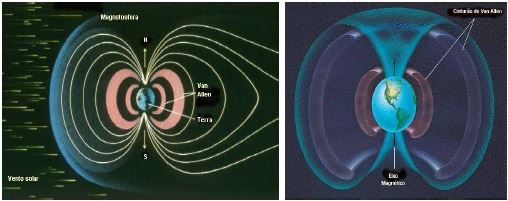
\includegraphics[width=0.7\textwidth]{figuras/cinturao.jpg}
	\caption[Cinturão de Van Allen]{Cinturão de Van Allen \cite{cinturao}.}
	\label{Img:cinturaoVanAllen}	
	%width=0.5\textwidth (Tamanho da Imagem)
\end{figure}

\subsection{Atividade Solar}

O sol é responsável por grande parte da radiação presente no espaço. A atividade solar segue uma variação regular e periódica com 11 anos de duração, e este período é comumente conhecido como ciclo solar. O ciclo solar é a recorrência de periódicas manchas solares na superfície do Sol. Durante o ciclo solar ocorre uma mudança periódica na energia solar, radiação e a ejeção de material solar \cite{Mansoori:2013}. O período de 11 anos correspondente ao ciclo solar está divido em aproximadamente 7 anos de alta atividade e 4 anos de baixa atividade \cite{Boudenot:2007}. 

Durante a baixa atividade solar o sol emite rajadas de partículas energéticas no espaço. Essas podem ser chamadas de erupções solares, que são compostas principalmente de prótons, com uma menor quantidade de partículas alfa (5\% a 10\%), íons pesados e elétrons, ou seja, as explosões solares emitem uma quantidade relativamente menor do que o fluxo de raios cósmicos que viajam pelo sistema solar.

Durante a alta atividade solar o sol emite uma quantidade maior de íons pesados podendo aumentar em até quatro ordens de grandeza, ou seja, o fluxo de íons é maior do que os observados para os raios cósmicos, por períodos que podem chegar a vários dias \cite{Stassinopoulos:1988}. 

A alta temperatura da coroa solar proporciona energia suficiente para que os elétrons escapem da atração gravitacional do sol. O efeito resultante da ejeção dos elétrons gera um desequilíbrio resultando numa ejeção de prótons e íons pesados da coroa solar. O vento solar é composto por aproximadamente 95\% de prótons, 4\% de íons de Hélio e 1\% de outros íons pesados e elétrons com uma quantidade necessária para tornar o vento solar neutro \cite{Velazco:2007}. 



\subsection{Raios Cósmicos} \label{subsec:raiosCosmicos}

O termo raio cósmico não possui uma definição científica clara. Ele tem sido utilizado desde o início do século XX para indicar as partículas energéticas que interferem com os estudos de materiais radioativos. Segundo Stassinopoulos e Raymond \cite{Stassinopoulos:1988} os raios cósmicos consistem em cerca de 85\% de prótons, cerca de 14 \% de partículas alfa, e cerca de 1\% de materiais mais pesados como, por exemplo, núcleo de carbono e ferro. Já Boudenot \cite{Boudenot:2007}, afirma que a composição dos raios cósmicos galácticos compreende 83\% de prótons, 13\% de núcleos de hélio e 3\% de elétrons. 

As Partículas produzidas na atmosfera da Terra surgem quando os raios cósmicos primários atingem átomos atmosféricos e criam uma chuva de partículas secundárias. Esses são também chamados de partículas em cascata. As partículas que finalmente atingem a terra são chamadas de partículas terrestres, menos de 1\% do fluxo primário atinge o nível do mar, e elas são na sua maioria compostas de múons, prótons, nêutrons e píons. A primeira observação de um \textit{Single Event Upset} (SEU) na superfície terrestre devido a raios cósmicos ocorreu no ano de 1979 \cite{ZieglerLandFord:1979}.


\subsection{Partículas alpha}

São compostas por dois nêutrons e dois prótons provenientes de um átomo de hélio duplamente ionizado a partir do decaimento nuclear de isótopos instáveis. No final da década de 70, as partículas alfa emitidas de materiais com traços de Urânio (U) e Tório (Th) foram mostradas como a causa dominante de um SEU numa memória \textit{RAM} na superfície terrestre \cite{Woods:1978}. Estas partículas estão presentes nos materiais utilizados para o encapsulamento de circuitos integrados, no qual é necessária uma baixa concentração de Urânio (U) e tório (Th) para reduzir a emissão e o equilíbrio de partículas alfa, mas não sendo o suficiente para eliminá-las. Em situações de não equilíbrio, foi destacado que o material utilizado no processo de solda dos dispositivos, usualmente feitos de cumbo (Pb) e estanho (Sn), os quais são extraídos de minérios que podem conter traços de Urânio (U) e Tório (Th) que causam a incidência de partículas alfa. Por isso é aconselhável que projetistas não posicionem pontos de solda próximos aos nós dos circuitos \cite{Velazco:2007}.


\subsection{Efeitos Singulares ou \textit{Single Event Effects}(SEE)} \label{subsec:EfeitosSingulares}

Efeitos singulares são causados por uma única partícula e podem assumir muitas formas. Estão associados a erros transientes num dispositivo causado pela indução de partículas energéticas ou radiação cósmica \cite{Yu:2008}. O impacto de uma única partícula ionizada da origem a pares de elétrons ao longo da trajetória da partícula por meio de um material semicondutor, SEE podem ser classificados em vários tipos como por exemplo:

\begin{itemize}
	\item \textit{Single Event Upsets}(SEU): Um SEU ocorre quando a incidência de uma partícula num dispositivo digital provoca mudanças indesejáveis no seu estado lógico, como por exemplo, a inversão de bits de elementos de memória. Esta inversão resulta de quando um pulso transitório incide num espaço de memória, esse efeito é visto como uma inversão do valor de armazenamento no \textit{flip-flop}, ou seja, um \textit{bit-flip} \cite{Normand:1996}.
	
	\item \textit{Single Event Transients}(SET): São variações temporárias na tensão de saída de corrente ou de um circuito
	devido à passagem de um íon pesado através de um dispositivo sensível, ou seja, pulso transiente que pode ou não ser capturado por um elemento de memória \cite{Ecoffet:1994}.
\end{itemize}

\section{Dependabilidade} \label{sec:denpendabilidade}

Segundo Laprie \cite{LaprieAcidente:1990}, dependabilidade indica a qualidade do serviço fornecido por um dado sistema e a confiança depositada no serviço fornecido. Do ponto de vista etimológico ao que diz respeito ao termo dependabilidade, do inglês \textit{dependability}, o termo confiabilidade, do inglês \textit{reability} seria mais apropriado: a capacidade de confiar. Apesar de que \textit{dependability} é sinônimo de \textit{reability} \cite{LaprieAcidente:1990}. 

Segundo Laprie e Weber \cite{LaprieAcidente:1990, Weber:2002} tolerância a falhas e dependabilidade não são propriedades de um sistema a que se possa atribuir diretamente valores numéricos. Mas todos os atributos da dependabilidade correspondem a medidas numéricas. Seus principais atributos são dependabilidade, confiabilidade, disponibilidade, segurança de funcionamento (\textit{safety}) e segurança (\textit{security}). Um resumo dos principais
atributos é mostrado na Tabela \ref{Img:atDenp}.     


\begin{table}[h]
	\centering
	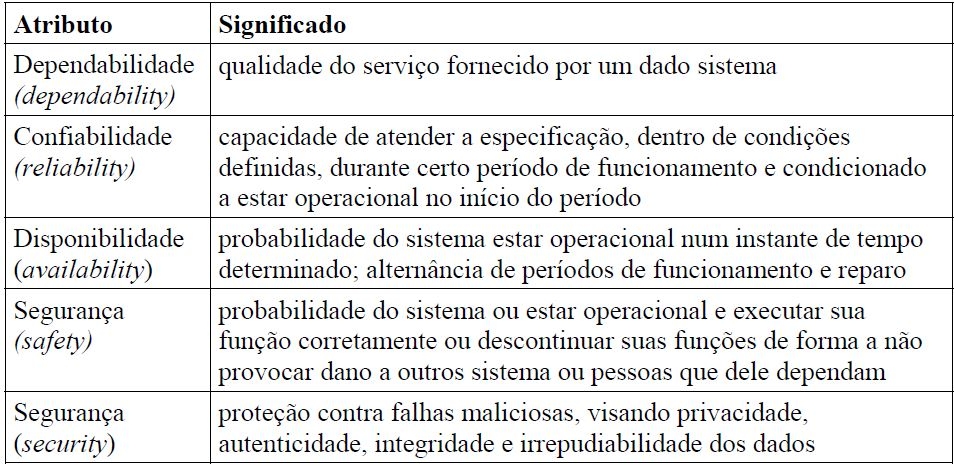
\includegraphics[width=0.7\textwidth]{figuras/tabelaDenpendabilidade.jpg}
	\caption[Resumo dos Atributos de Denpendabilidade]{Resumo dos atributos de dependabilidade Retirado de Weber \cite{Weber:2002}.}
	\label{Img:atDenp}	
	%width=0.5\textwidth (Tamanho da Imagem)
\end{table}



\section{Tolerância a Falhas} \label{sec:tolerancia}

Segundo Avizienis \cite{Avizienis:1984} quando um sistema é capaz de automaticamente se recuperar de erros causados por falhas, e eliminar uma falha sem sofrer um defeito externamente perceptível, diz-se que este sistema é tolerante a falhas. Na construção dos primeiros computadores, estratégias para construção de sistemas mais confiáveis já eram utilizadas para tolerar possíveis falhas \cite{VonNewmann:1956}. Apesar de envolver técnicas e estratégias tão antigas, a tolerância a falhas ainda não é uma preocupação rotineira de projetistas e usuários, ficando sua aplicação quase sempre restrita a sistemas críticos e mais recentemente a sistemas de missão crítica \cite{Weber:2002}.

Um aspecto importante em tolerância a falhas é a descrição das características das falhas. Há um conjunto de atributos que são utilizados para cumprir esta finalidade; são eles: causa, natureza, duração, extensão e valor. Na figura \ref{Img:falhasCaracteristicas} é mostrado os atributos das características das falhas.

Pêgo \cite{Pego:2014} descreve os conjuntos de atributos utilizados para caracterizar uma falha:

\begin{figure}[H]
	\centering
	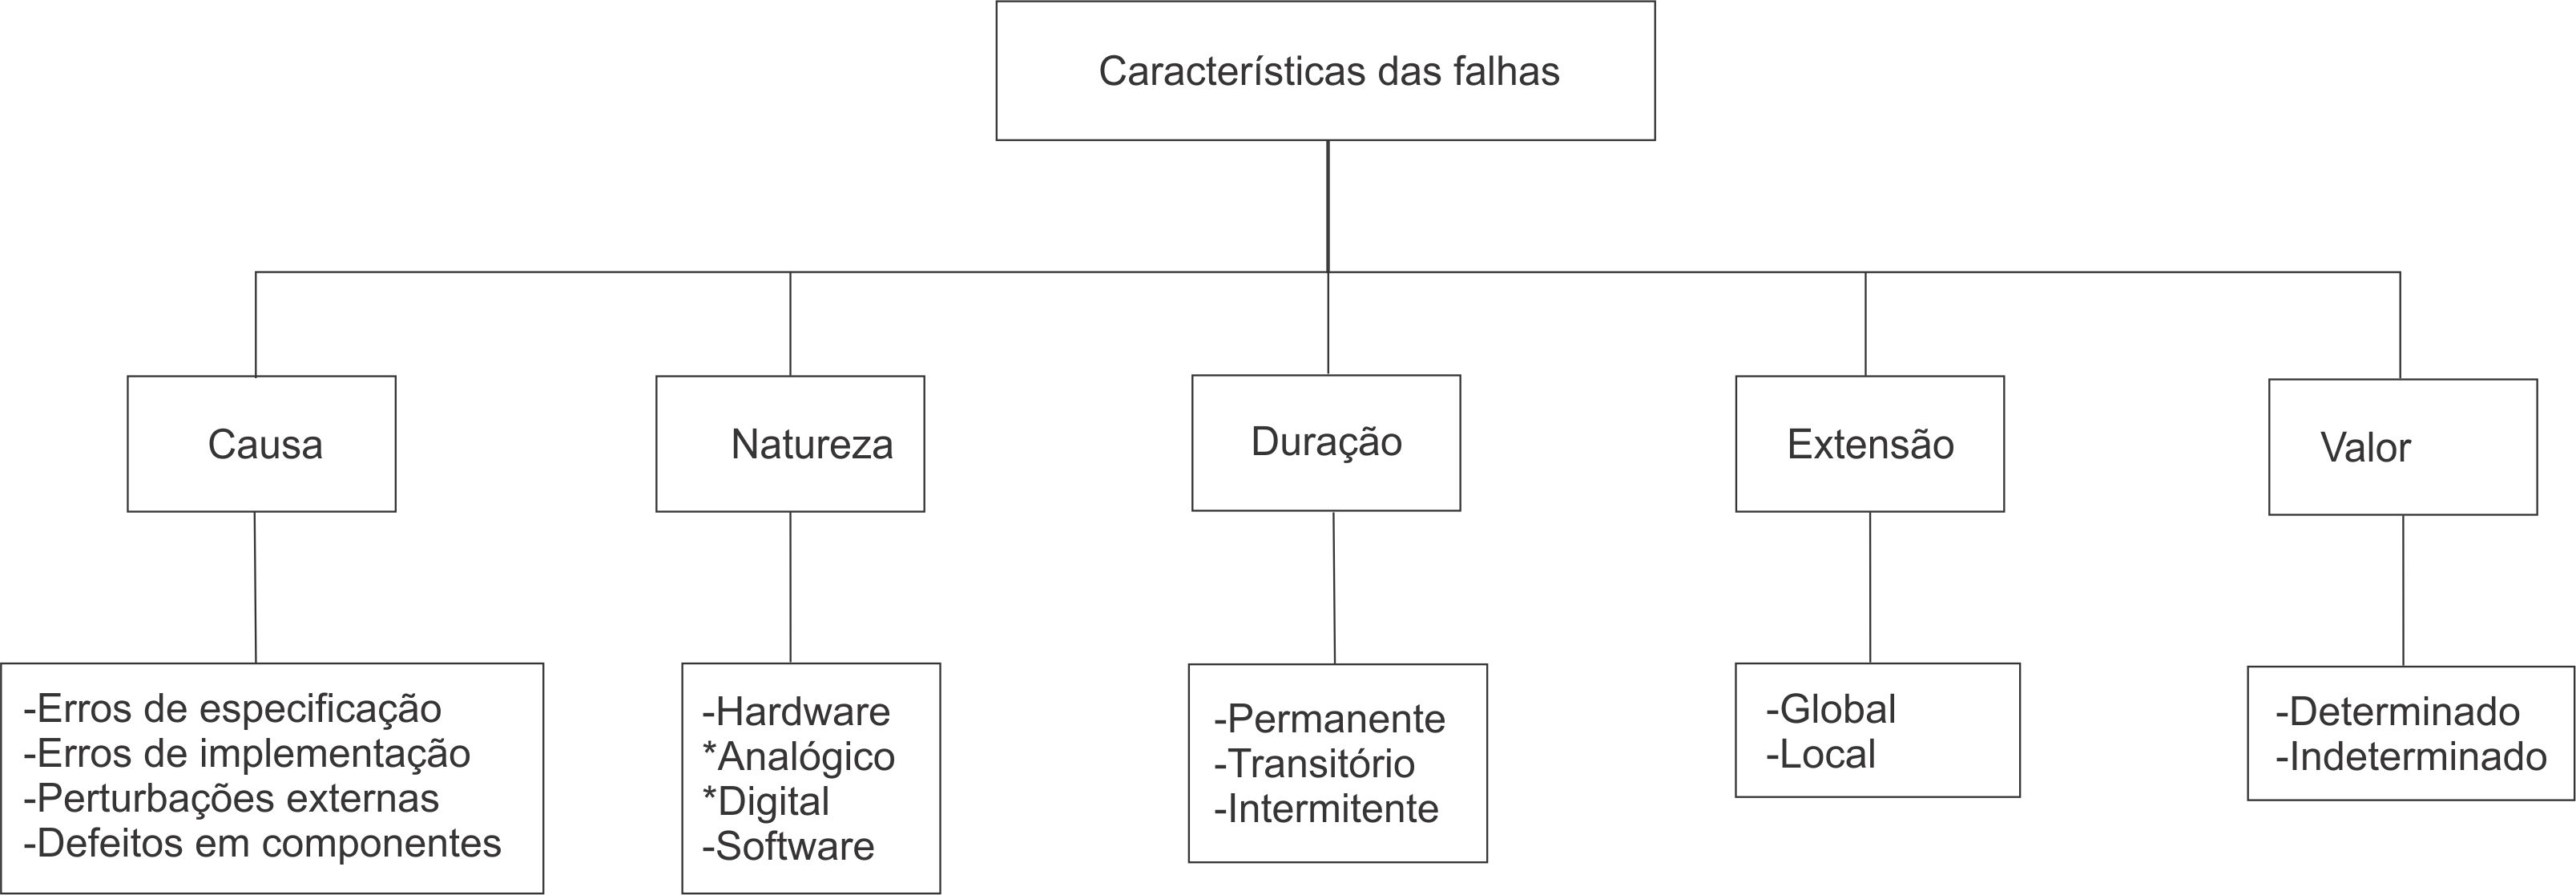
\includegraphics[width=0.7\textwidth]{figuras/falhasCaracteristicas.jpg}
	\caption[Características das Falhas]{Atributos das características das falhas. Retirado de Pego \cite{Pego:2014}.}
	\label{Img:falhasCaracteristicas}	
	%width=0.5\textwidth (Tamanho da Imagem)
\end{figure}

\begin{itemize}
	\item \textbf{Causa} - Uma falha pode ter origem em problemas de especificação, problemas de execução, defeitos em componentes do sistema operacional (que não são incomuns para dispositivos eletrônicos), ou em fatores externos, tais como, tempestades, poeira, temperatura, etc.
	
	\item \textbf{Natureza} - Uma falha pode ser proveniente de \textit{software} ou \textit{hardware}. Neste último, a falha pode estar na parte analógica, por exemplo, em transdutores e amplificadores, ou na parte digital, por exemplo, na unidade lógica Aritmética (ULA).
	
	\item \textbf{Duração} - Uma falha pode ser constante, o que significa que uma vez que os dados tenham sido persistidos no sistema, a falha continuará até que a manutenção adequada seja feita. Pode ainda ser transitória, quando ocorre em um período de tempo e logo em seguida, desaparece. Esse tipo de falha é geralmente provocada por causas externas. Relâmpago, por exemplo, podem provocar um erro súbito em um dispositivo, mas após o relâmpago, o dispositivo voltará ao seu funcionamento normal. Finalmente, há falhas, que são chamadas intermitentes; essas ocorrem em períodos curtos de tempo e desaparecem, mas depois elas voltam novamente. É possível que este processo se repita indefinidamente. Uma falha intermitente é a ocorrência de repetição de falhas transitórias.
	
	\item \textbf{Extensão} - A ocorrência de uma falha pode estar limitada a um escopo global ou local. Ou seja, uma falha pode afetar todo o sistema ou ser limitada a um determinado bloco. 
	
	\item \textbf{Valor} - O valor de uma falha pode ser determinado ou indeterminado. Ou seja, os valores relativos de uma falha podem ser constantes ou não. Na Seção \ref{sec:falhaErroDefeito} é citado um exemplo de uma falha que mantém um endereço de memória com um valor fixo em zero, este exemplo é chamado de valor determinado. Outra falha sem esta característica é chamada de indeterminada.
	
	
	
\end{itemize}


\section{Técnicas de Tolerância a Falhas}\label{sec:tecnica}

Para mitigar(abrandar, minimizar) os efeitos citados na Subseção \ref{subsec:EfeitosSingulares} e na Seção \ref{sec:falhaErroDefeito} são utilizadas técnicas de tolerância a falhas, nas quais envolvem alguma forma de redundância.  
Existem técnicas baseadas em \textit{software} e \textit{hardware}, neste trabalho foram citados apenas as técnicas baseadas em \textit{software}, pois no desenvolvimento da aplicação proposta não foram utilizadas as técnicas baseadas em \textit{hardware}, pois esta técnica demanda da utilização de um equipamento que realiza o bombardeamento de íons sobre o circuito eletrônico podendo danificar o \textit{hardware} \cite{Weber:2002}.

\subsection{Técnicas de redundância baseadas em software}

Segundo Pêgo \cite{Pego:2014} a inserção de redundância no código ou nos dados permite que seja possível detectar e até mesmo corrigir eventuais falhas. A inserção de instruções pode ser feita em programas escritos tanto em liguagem C, \textit{assembly} e até em níveis mais baixos, a redundância temporal em nível de intruções pode ser dividida em:


\begin{itemize}
	\item \textbf{Técnicas orientadas a dados} - Cada dado armazenado é replicado em cada operação, na checagem da consistência dos dados sendo necessária a alteração do código fonte. Pode ser implementado em linguagens de baixo nível como C, que será utilizada neste trabalho, \textit{assembly} e até no código intermediário gerado pelo compilador \cite{Pego:2014}.
	
	\item \textbf{Técnicas orientadas ao controle} - As falhas que podem modificar o fluxo correto de execução dos programas são detectadas e tratadas. Todas as técnicas no nível de instrução são baseadas na divisão do código do programa em blocos, construção de grafos e a checagem em tempo de execução sobre a correta transição entre os vértices deste grafo \cite{Pego:2014}.  		 
	
\end{itemize}


Weber \cite{Weber:2002} afirma que a simples replicação de componentes idênticos é uma estratégia de detecção e mascaramento de erros inútil em \textit{software}. Componentes idênticos de \textit{software} vão apresentar erros idênticos. Assim não basta copiar um programa e executá-lo em paralelo ou executar o mesmo programa duas vezes em tempos diferente. Erros de programas idênticos vão apresentar, com grande probabilidade, de forma idêntica para os mesmos dados de entrada. Segundo Brilliant \textit{et al.}\cite{Brilliant:1990} outras formas de redundância de \textit{software} como, por exemplo, diversidade ou programação n-versões, blocos de recuperação e variação de consistência não envolvem cópias idênticas.

\subsection{Diversidade ou Programação N-Versões}

A partir de um problema, são implementadas diversas soluções alternativas, sendo a reposta do sistema determinada por votação, esta técnica é ilustrada na Figura \ref{Img:nVersion}. Segundo Avizienis \cite{Avizienis:1995} A. \textit{apud} Fischler et. al., os esforços de programação são realizados por \textit{n} indivíduos. Sempre que for possível, diferentes algoritmos e linguagens de programação são usados em cada versão. Cada versão do programa é implementada de forma independente com base na especificação inicial do problema, embora sejam diferentes na sua implementação, as N-versões são funcionalmente equivalentes e dificilmente apresentarão as mesmas falhas \cite{Avizienis:1995}. 

\begin{figure}[H]
	\centering
	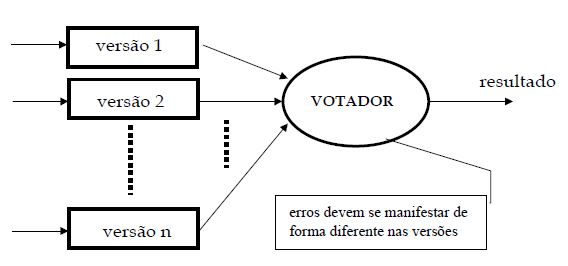
\includegraphics[width=0.7\textwidth]{figuras/nVersions.jpg}
	\caption[Programação N-Versões]{Diversidade ou Programação N-Versões. Retirado de Weber \cite{Weber:2002}.}
	\label{Img:nVersion}	
	%width=0.5\textwidth (Tamanho da Imagem)
\end{figure}  

Um exemplo de programação n-versões é o sistema de bordo do \textit{Space Shutle}, no qual quatro computadores idênticos são utilizados em NMR (\textit{N-Modular Redundancy}). Esta técnica consiste em replicar o \textit{hardware} responsável pelo processamento da informação em \textit{n} módulos. Um quinto computador com \textit{hardware} diferente dos outros quatro, pode substituir os demais em caso de colapso no esquema NMR \cite{Pradhan:1996}.

\subsection{Blocos de Recuperação}

Nesta técnica são utilizados testes de aceitação, no qual programas serão executados um a um até que o primeiro passe no teste de aceitação. A técnica de blocos de recuperação é semelhante a programação n-versões, mas nessa técnica programas secundários só serão necessários na detecção de um erro no programa primário. Esta técnica tolera n-1 falhas, no caso de falhas independentes nas \textit{n} versões \cite{Nelson:1990, Weber:2002, Somani:1997}.   

\begin{figure}[H]
	\centering
	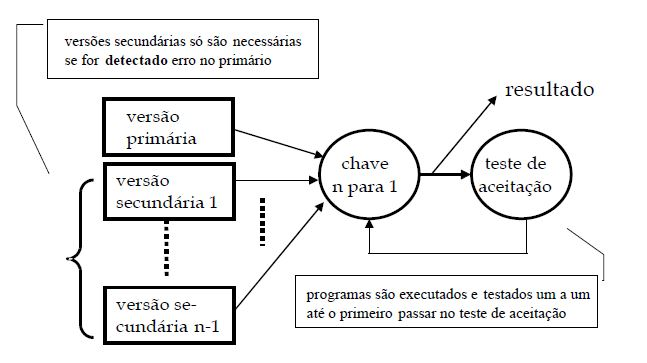
\includegraphics[width=0.7\textwidth]{figuras/blocoRecuperacao.jpg}
	\caption[Blocos de Recuperação]{Blocos de Recuperação. Retirado de Weber \cite{Weber:2002}.}
	\label{Img:blocoRecuperacao}	
	%width=0.5\textwidth (Tamanho da Imagem)
\end{figure}


\subsection{Verificação de Consistência}

É uma ampliação da programação n-versões. Nessa técnica também são utilizadas \textit{n} equipes, assim como na programação n-versões, que implementam soluções independentes a partir de uma única especificação, no entanto, as equipes também desenvolvem um módulo específico para verificar a saída dos dados de seu próprio sistema em tempo real e compará-los com uma base de informações prévia para apurar a corretude da informação. Os \textit{softwares} das equipes são executados paralelamente e as saídas são submetidas a verificação. A saída passa a ser verificada em seu próprio módulo e o resultado é definido pelo primeiro módulo que passar ou por um sistema de votação \cite{Nelson:1990,Kruger:2014}.

\section{Injeção de Falhas} \label{sec:InjecaoDeFalhas}

A injeção de falhas é um processo importante para validar e verificar a confiabilidade de um sistema, seja por alteração de código, simulando uma falha de \textit{software} \cite{Kanawati:1995} ou a nível de pinos (\textit{Pin-level Injection}) injetando falhas diretamente no \textit{hardware} \cite{Arlat:2003}. Além da injeção de  falhas por \textit{software} e por \textit{hardware} existe um terceiro tipo chamado injeção de falhas por Simulação. Arlat \cite{Arlat:2003} afirma que injeção de falhas baseadas em simulação se restringem aos modelos de alto nível, como por exemplo os modelos VHDL (\textit{VHSIC Hardware Description Language}) Linguagem de descrição de \textit{hardware} de circuitos de alta velocidade. 

Segundo Arlat \textit{et. al.} \cite{Arlat:1990} a validação e auxílio de projeto são as duas metas principais que compõem o método de injeção de falhas. Com um conjunto de testes a validação dos procedimentos de verificação são utilizados para descobrir falhas durante todo o processo de desenvolvimento. A validação dos mecanismos de tolerância a falhas é usada para detecção e recuperação de falhas com o objetivo de alcançar a dependabilidade do sistema na fase operacional. É importante ressaltar dois aspectos importantes na validação, que é a previsão de falhas, na qual os mecanismos de manipulação de falhas são avaliados em sua eficiência na estimação de medidas como cobertura e latência \cite{Arlat:1990}.

O auxílio ao projeto ocorre durante a fase de desenvolvimento do projeto, buscando melhorar a eficiência dos mecanismos de testes e o protocolo de tolerância a falhas por meio da injeção de falhas \cite{Arlat:1990}.

Uma das vantagens da utilização do método de injeção de falhas está no fato de ser uma técnica que permite a avaliação de um protótipo de sistema sob falhas, em particular ela mede a eficácia da detecção de erros do sistema e sua capacidade de correção. Outra vantagem são os efeitos das falhas no sistema que permitem revelar falhas críticas que por ventura viessem a ocorrer na execução do sistema em um ambiente real \cite{Arlat:2003}.     

\subsection{Injeção de falhas por \textit{Hardware}}

Esta técnica necessita de um \textit{hardware} especial, no qual as falhas seriam originadas. Arlat \cite{Arlat:2003} apresenta algumas ferramentas para injeção de falhas por \textit{hardware} como \textit{MESSALINE}, \textit{RIFLE} E \textit{AFIT}, todas utilizadas para injeção de falhas a \textit{pin-level}, que consiste na injeção de falhas por meio de pinças ou posicionando o circuito sobre soquetes conectados a um injetor de falhas \cite{Arlat:1990, Arlat:2003}. Outras técnicas de injeção de falhas por \textit{hardware} são interferências eletromagnéticas e irradiação de íons pesados \cite{Gunnelo:1989, Arlat:1990, Arlat:2003}, estas por sua vez podem danificar o componente sob teste \cite{Sotoma:1997}. O objetivo dessas técnicas visa principalmente estudar o comportamento dos mecanismos de tolerância a falhas implementados por \textit{hardware}, porém também se pode testar os mecanismos de falhas por meio de \textit{softwares} que não danificam os componentes sob teste \cite{Martins:1989}.


\subsection{Injeção de falhas por \textit{Software}}

Esta técnica visa modificar o estado do \textit{hardware/software} do sistema por meio de um programa, fazendo com que o sistema se comporte como se uma falha de \textit{hardware} estivesse ocorrendo. Pode-se emular falhas em vários níveis do sistema desde que a funcionalidade do \textit{hardware} esteja visível através do \textit{software}. Por isso, injetar falhas por \textit{software} é menos dispendioso em termos de tempo e esforço do que as técnicas de \textit{hardware} implementadas, devido a capacidade de alterar o estado de registradores e memória \cite{Kanawati:1995}. Um exemplo de injeção de falhas por \textit{software} é a ferramenta \textit{Ferrari} apresentada por Kanawati \textit{et. al.} \cite{Kanawati:1995} que possibilita a injeção de falhas transitórias, bem como falhas permanentes, de modo que ele possa verificar a eficácia da detecção de erros e a correção simultânea dos mecanismos de verificação de falhas, e a capacidade para executar a injeção em código aberto. Alguns exemplos de injetores de falhas são FERRARI \cite{Kanawati:1995}, PFI \cite{Dawson:1995}, SFI \cite{Rosenberg:1993} e FIAT \cite{Segall:1988}. 


\section{\textit{Design Patterns}} \label{sec:designPattern}
				
Neste trabalho foi necessário a utilização de \textit{design patterns} (padrões de projeto) para a elaboração de códigos eficientes. A ideia básica dos padrões de projeto é a de utilizar soluções conhecidas para problemas conhecidos. Cada padrão de projeto descreve um problema e sua solução, com isso, terceiros podem a utilizar sem ter a necessidade de descobri-la novamente, economizando tempo e padronizando o desenvolvimento do projeto \cite{Vinicius:2009}. Em geral, \textit{design patterns} possuem alguns elementos que facilitam no desenvolvimento da sua aplicação \cite{Engholm:2010}, são eles:

\begin{itemize}
	\item \textbf{Contexto} - Situação na qual o problema está sendo endereçado corretamente.
	
	\item \textbf{Problema} - Problema de design para o qual o padrão se destina.
	
	\item \textbf{Necessidade} - Quesitos de design para o qual o padrão se destina.
	
	\item \textbf{Solução e estrutura} - Solução do problema.
	
	\item \textbf{Consequências} - Vantagens e desvantagens de se utilizar o padrão.
	
	\item \textbf{Padrões associados} - Padrões similares ou utilizados para construir o padrão.
\end{itemize}

\subsection{Padrão GoF (Padrões Fundamentais Originais)} \label{subsec:gof}

O conceito de máquina de estados foi utilizado neste trabalho  para o desenvolvimento da biblioteca \textit{FaultRecovery}. O padrão \textit{State} vai ao encontro da resolução deste problema.

Os padrões GoF são divididos em três grupos: padrões de comportamento, de criação e estruturais. Estes descrevem como os objetos devem ser gerenciados pelas estruturas de um programa, esses fornecem maneiras robustas de se criar objetos, e aqueles descrevem como os objetos interagem, distribuindo responsabilidades \cite{Engholm:2010}. Neste trabalho utilizou-se o padrão \textit{State}, indicado para programas que podem ser representados por uma máquina de estados, que é o caso dos \textit{firmwares} desenvolvidos para o microcontrolador \textit{mbed}. O padrão \textit{State} faz parte dos padrões de comportamento e permite que parte do comportamento de um objeto seja alterado conforme o estado do objeto. Cada objeto possui atributos, que representam seu estado, e também métodos, que representam seu comportamento \cite{Vinicius:2009}.